% Journal of Computational Sciences
%\documentclass[3p]{elsarticle}

% APS journals: PRL and PRF
% Note: All AIP and APS journals use the revtex package; both PRL and PRF are APS.
\documentclass[reprint, superscriptaddress, notitlepage]{revtex4-1}

% PACKAGES
\usepackage{graphicx, amsmath, amssymb, amsfonts, mathtools, mathrsfs, color}
\usepackage{comment, enumerate, tabularx, multirow}
\usepackage{natbib, hyperref, url}
\usepackage{algorithm, algpseudocode, pifont, longtable}
%\usepackage[justification=RaggedRight]{caption}


%^^^^^^^^^^^^^^^^^^^^^^^^^^^^^^^^^^^^^^^^^^^^^^^^^^^^^^^^^^^^%
% COMMANDS
% Basic editing
\newcommand{\tocite}{{\color{blue}(to cite)}}
\newcommand{\vsp}[1]{\vspace{#1 pc} \noindent}
\newcommand{\np}{\newpage \noindent}
\newcommand{\HERE}[1]{ \vsp{#1} {\color{blue} HERE} }
\newcommand{\tofix}{\color{blue}}
\newcommand{\new}{}		% \color{green}
\newcommand{\newa}{}		% \color{red}
\newcommand{\newb}{}		% \color{blue}
% Basic math, derivatives
\newcommand{\td}[2]{\frac{d #1 }{d #2}}
\newcommand{\ttd}[2]{\frac{d^2 #1 }{{d #2}^2}}
\newcommand{\pd}[2]{ \frac{ \partial #1}{ \partial #2 } }
\newcommand{\ppd}[2]{ \frac{ \partial^2 #1}{ {\partial #2}^2 } }
% Basic math, vectors and other
\newcommand{\BigO}[1]{ \mathcal{O} \left(#1\right) }
\newcommand{\bvec}[1]{\ensuremath{\boldsymbol{#1}}}
\newcommand{\grad}{\nabla} 
\newcommand{\abs}[1]{\left| #1 \right|}
\newcommand{\tavg}[1]{\langle #1 \rangle}
\newcommand{\norm}[1]{ \left\| #1 \right\| }
\newcommand{\ip}[1]{ \langle #1 \rangle }
% For real and imaginary, could use \Re or \Im, or \mathcal{R}, or \text{Re}
%^^^^^^^^^^^^^^^^^^^^^^^^^^^^^^^^^^^^^^^^^^^^^^^^^^^^^^^^^^^^%


%^^^^^^^^^^^^^^^^^^^^^^^^^^^^^^^^^^^^^^^^^^^^^^^^^^^^^^^^^^^^%
% TITLE AUTHORS ABSTRACT
\begin{document}
\title{Fluid-mechanical erosion generates anisotropy in porous media}
%\title{Erosion leads to anisotropy in a porous medium}
%\title{The development of anisotropy in an eroding porous medium}
%

\author{M.~N.~J.~Moore}
\affiliation{Department of Mathematics and Geophysical Fluid Dynamics Institute, Florida State University, Tallahassee, FL, 32306.}
\author{Bryan D.~Quaife}
\affiliation{Department of Scientific Computing and Geophysical Fluid Dynamics Institute, Florida State University, Tallahassee, FL, 32306.}
\author{Shang-Huan Chiu}
\affiliation{Department of Scientific Computing, Florida State
University, Tallahassee, FL, 32306.}

\begin{abstract}
We numerically simulate the erosion of a porous medium due to an internally flowing fluid. The solid constituents of the porous medium erode under the action of surface shear stress. As the particles shrink, they elongate in the direction of the flow, giving rise to anisotropic conductivity of the porous medium.
\end{abstract}
\maketitle
%^^^^^^^^^^^^^^^^^^^^^^^^^^^^^^^^^^^^^^^^^^^^^^^^^^^^^^^^^^^^%

\section{Introduction}

Effects of flow-induced erosion are visible across a range of scales in nature, from massive geological structures, to mesoscopic patterns, and finally down to the tiny granular constituents that comprise a porous medium. In the case of a porous medium specifically, it has been long recognized that bulk properties of mediums encountered in nature are typically anisotropic, so that the medium allows flow in a preferred direction more easily. This anisotropy is commonly attributed to how grains are deposited, with their longest dimension parallel to the settling bed, so that they allow flow preferentially in the horizontal direction. Controlled experiments, however, have not been performed to test this hypothesis. Here, we use highly-accurate numerical simulations to examine an alternative, and possibly complementary, mechanism: namely, that the flow-induced erosion of the medium's solid constituents contributes to its overall anisotropy.

Our method merges highly-efficient and highly-accurate boundary-integral methods with stable interface evolution methods to simulate the erosion of many solid-bodies in Stokes flow---the regime of groundwater flow. This method is documented, validated, benchmarked in \cite{Quaife2018}, and can practically simulate the erosion of order hundreds of solid bodies.


%Stuff to cite \cite{Ristroph2012, Moore2013, Huang2015, MooreCPAM2017} and other stuff \cite{Rycroft2016, Mitchell2016}.


\begin{comment}
%^^^^^^^^^^^^^^^^^^^^^^^^^^^^^^%
\begin{figure}%[htbp]
\begin{center}
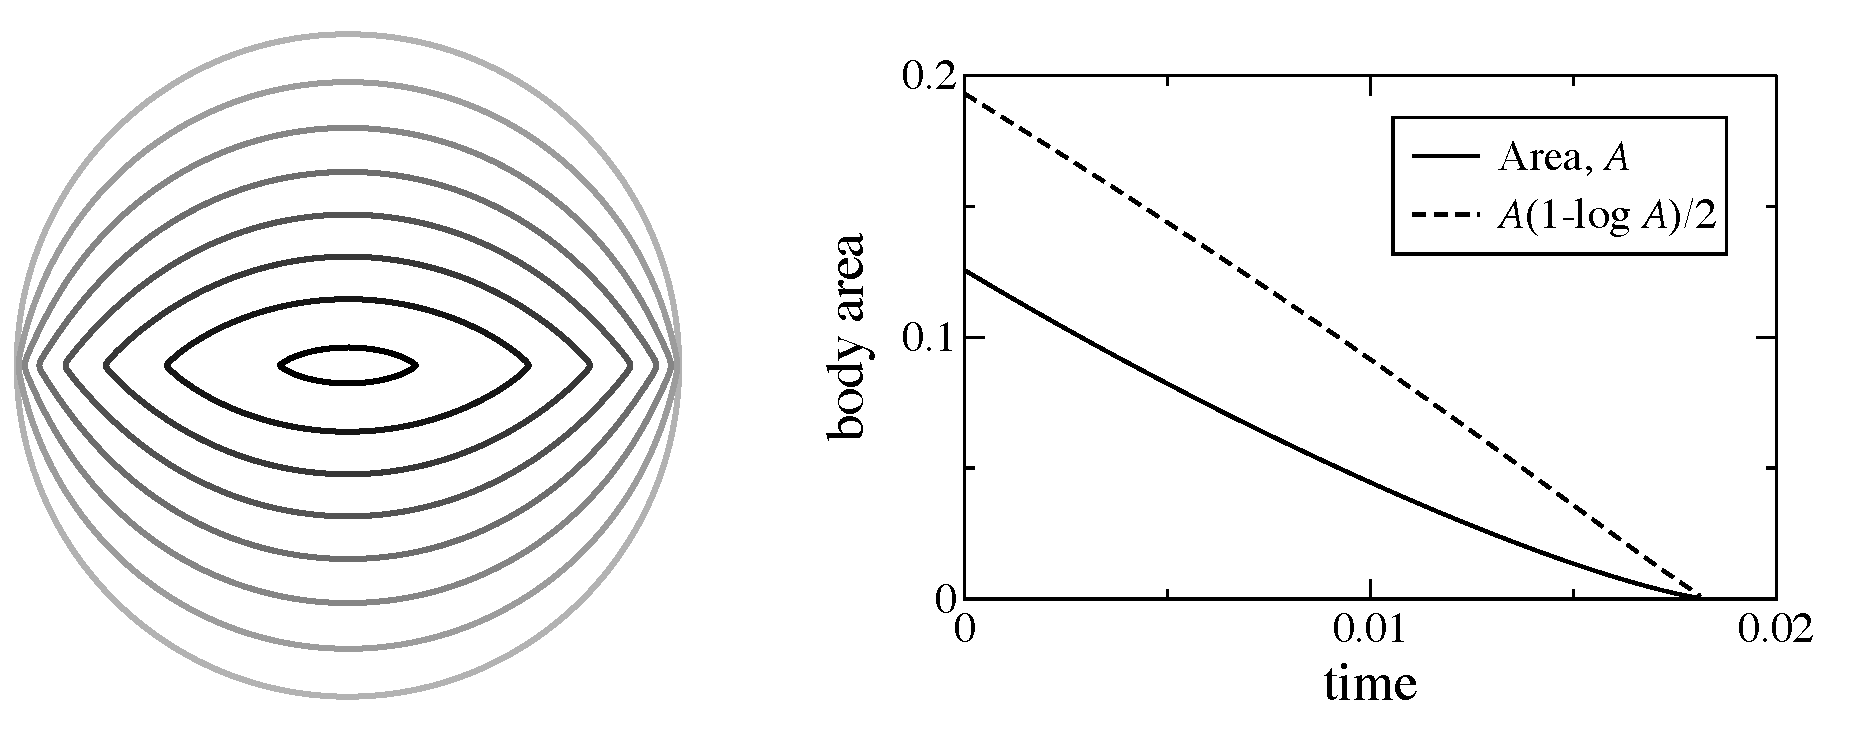
\includegraphics[width = 0.9 \textwidth]{./Figs/fig1.pdf}
\caption{caption}
\label{fig1}
\end{center}
\end{figure}
 %^^^^^^^^^^^^^^^^^^^^^^^^^^^^^^%

%^^^^^^^^^^^^^^^^^^^^^^^^^^^^^^%
\begin{figure}%[htbp]
\begin{center}
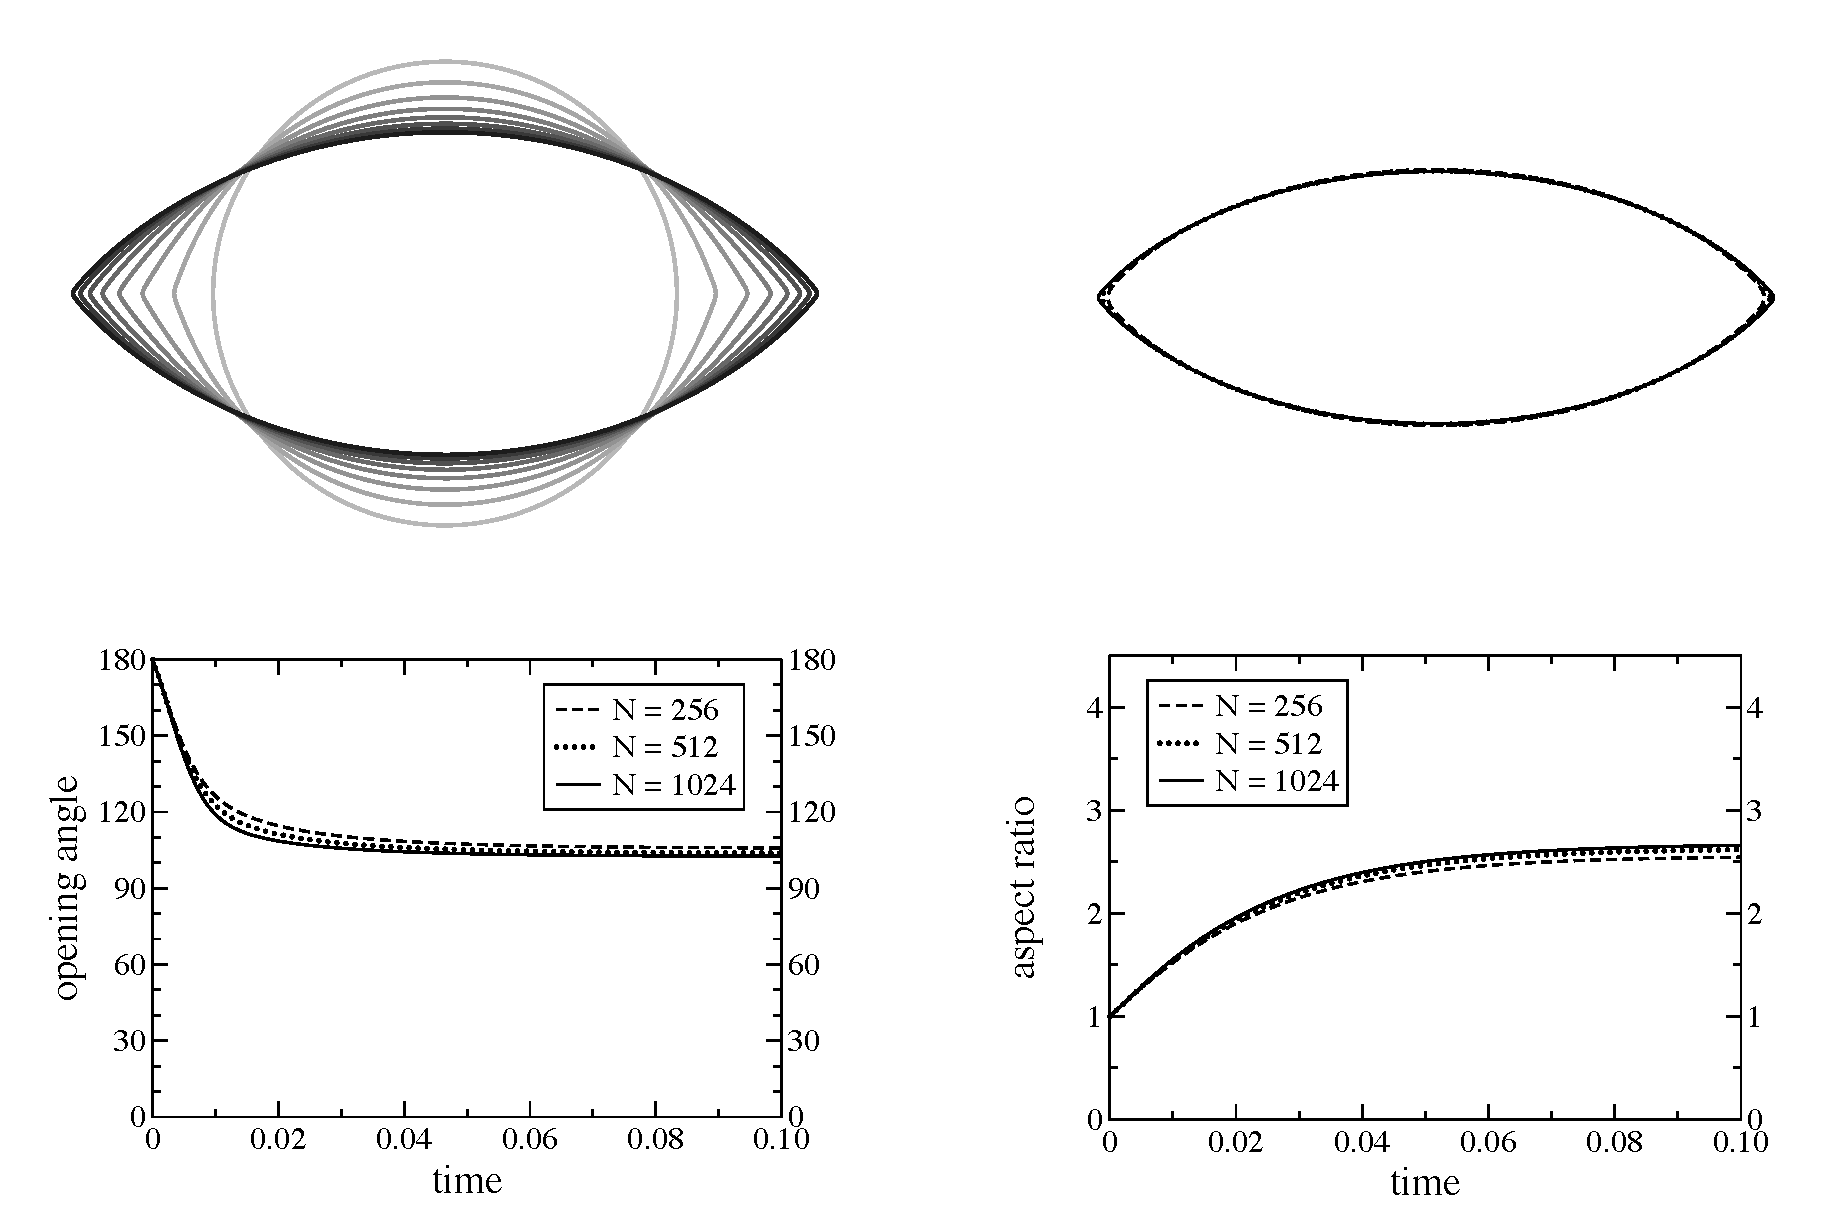
\includegraphics[width = 0.9 \textwidth]{./Figs/fig2.pdf}
\caption{caption}
\label{fig2}
\end{center}
\end{figure}
 %^^^^^^^^^^^^^^^^^^^^^^^^^^^^^^%
\end{comment}


\bibliographystyle{plain}
\bibliography{refs}
\end{document}
